\documentclass[11pt]{article}
\usepackage[margin=1in]{geometry}
\usepackage{amsmath,amssymb}
\usepackage{booktabs}
\usepackage{tabularx}
\usepackage{graphicx}
\usepackage{xcolor}
\usepackage{hyperref}
\usepackage{enumitem}
\setlist{nosep,leftmargin=*}
\hypersetup{colorlinks=true,linkcolor=blue!50!black,urlcolor=blue!50!black}
\newcommand{\SMB}{\textsc{smb}}
\newcommand{\HML}{\textsc{hml}}
\newcommand{\MOM}{\textsc{mom}}

\title{STA348 Term Project: Factor-Leadership HMM\\[4pt]\large Data Diagnostics --- Sources, Cleaning, Sample Split and Summary Statistics}
\author{Richard}
\date{November 2026}

\begin{document}
\maketitle

\begin{abstract}
\noindent This document records the data behind the factor-leadership hidden Markov model: the raw Ken French files, every cleaning and alignment step, the number of observations kept and dropped at each step, the chronological train/test split, and summary statistics for the three factors and for the encoded top-factor sequence. Two datasets are used: monthly (1{,}197 months, January 1927 -- September 2026) and weekly (5{,}212 weeks, November 1926 -- September 2026). No missing values were found; the only observations dropped are periods before momentum data begin and three trailing days after the last published week.
\end{abstract}

\tableofcontents

%==========================================================================
\section{Raw sources}

All factor data come from the Kenneth R.\ French Data Library, built from the CRSP database vintage \textbf{202609} (stated in each file header). Values are monthly, weekly or daily returns in percent.

\begin{center}
\small
\begin{tabularx}{\textwidth}{@{}lXrrll@{}}
\toprule
File & Contents used & Data rows & Annual rows & First & Last \\
\midrule
\texttt{F-F\_Research\_Data\_Factors} (monthly) & \SMB, \HML{} & 1{,}203 & 99 & 1926-07 & 2026-09 \\
\texttt{F-F\_Momentum\_Factor} (monthly) & \MOM & 1{,}197 & 99 & 1927-01 & 2026-09 \\
\texttt{F-F\_Research\_Data\_Factors\_weekly} & \SMB, \HML{} & 5{,}230 & --- & 1926-07-02 & 2026-09-25 \\
\texttt{F-F\_Momentum\_Factor\_daily} & \MOM & 26{,}237 & --- & 1926-11-03 & 2026-09-30 \\
\bottomrule
\end{tabularx}
\end{center}
The market excess return (Mkt-RF) and risk-free rate (RF) are read but not used by the model.

\textbf{Factor definitions.} \SMB{} (small minus big) and \HML{} (high minus low book-to-market) come from six value-weighted portfolios formed each June on size and book-to-market. \MOM{} is the average return of the two high prior-return portfolios minus the two low prior-return portfolios from a $2\times3$ size by prior-return sort. All three are zero-investment long--short returns.

\textbf{Two momentum constructions.} The monthly file re-forms portfolios monthly using returns from month $-12$ to $-2$; the daily file re-forms them daily using day $-250$ to $-21$. The weekly dataset uses the daily file (there is no weekly momentum file), so weekly and monthly \MOM{} are related but not identical series (Section~\ref{sec:checks}).

%==========================================================================
\section{Cleaning and alignment method}

\subsection{Parsing (all files)}
\begin{enumerate}
\item Read the CSV directly or from inside the downloaded \texttt{.zip}.
\item Skip the text preamble. The data block starts after the header line beginning with a comma (e.g.\ \texttt{,Mkt-RF,SMB,HML,RF}).
\item Keep rows whose first field is a date: \texttt{YYYYMM} (monthly) or \texttt{YYYYMMDD} (weekly, daily). The block ends at the first non-data line, which excludes the \emph{annual} table appended to the monthly files (99 rows each).
\item Monthly dates are set to the last calendar day of the month; weekly and daily dates are used as given.
\item Missing-value codes ($-99.99$, $-999$) are converted to missing. \textbf{None occur} in the data rows of any file used (the code appears only in the momentum file's description text).
\item Divide by 100 to convert percent to decimals.
\end{enumerate}

\subsection{Monthly dataset}
The monthly \SMB/\HML{} file and the monthly \MOM{} file are joined on month (inner join), keeping months present in both.

\subsection{Weekly dataset}
French publishes weekly \SMB{} and \HML{} but no weekly \MOM. Daily \MOM{} is compounded into French's own weeks so that all three factors cover the same trading days:
\begin{enumerate}
\item Let $w_1<w_2<\dots$ be the weekly dates in the 3-factor file (the last trading day of each week).
\item Assign each daily momentum date $d$ to the first weekly date on or after it, $w(d)=\min\{w_i: w_i\ge d\}$.
\item Compound within each week: $\MOM^{\text{week}}_{w}=\prod_{d:\,w(d)=w}\big(1+\MOM^{\text{day}}_d\big)-1$.
\item Join with weekly \SMB, \HML{} (inner join).
\item Drop the first week if it contains fewer than four momentum days (it contains four, so it is kept).
\end{enumerate}

\subsection{Observation encoding}
Each period's observation is the factor with the highest return,
\[
o_t=\arg\max_{k\in\{\SMB,\HML,\MOM\}} f_{k,t},\qquad 0=\SMB,\ 1=\HML,\ 2=\MOM,
\]
where $f_{k,t}$ is factor $k$'s return in period $t$ (decimal). Exact ties are resolved in favour of the first factor in the order \SMB, \HML, \MOM{} (\texttt{numpy.argmax}); Section~\ref{sec:encoding} shows ties are negligible.

\subsection{Optional volatility scaling}
When enabled, $f_{k,t}$ is replaced by $f_{k,t}/\hat\sigma_{k,t-1}$, the return divided by its standard deviation over the previous 36 months or 52 weeks (lagged one period). The first 36 months or 52 weeks are lost to the window. This variant is not used in the main results.

%==========================================================================
\section{Observations kept and dropped}

\begin{center}
\small
\begin{tabularx}{\textwidth}{@{}Xrrl@{}}
\toprule
Step & Monthly & Weekly & Notes \\
\midrule
3-factor file, data rows & 1{,}203 & 5{,}230 & \\
Momentum file, data rows & 1{,}197 & 26{,}237 days & weekly: daily file \\
Dropped: before momentum starts & 6 & 18 & Jul--Dec 1926 / Jul--Oct 1926 \\
Dropped: momentum days after last week & --- & 3 days & 28--30 Sep 2026 \\
Dropped: missing values & 0 & 0 & \\
Dropped: duplicates & 0 & 0 & \\
\midrule
\textbf{Final sample} & \textbf{1{,}197} & \textbf{5{,}212} & \\
Vol-scaled variant (after window) & 1{,}161 & 5{,}160 & first 36 / 52 periods lost \\
\bottomrule
\end{tabularx}
\end{center}

\subsection{Calendar integrity}
\textbf{Monthly:} no gaps; every calendar month from January 1927 to September 2026 is present once.

\textbf{Weekly:} gaps between consecutive weekly dates are 7 days in 4{,}820 of 5{,}211 cases; shorter or longer gaps reflect holidays moving the last trading day (e.g.\ Thursday before Good Friday) and are French's own week definitions. Weekly dates fall on Friday (3{,}914), Saturday (1{,}142; Saturday trading before 1952), Thursday (152), Wednesday (3) and Monday (1).

\begin{center}
\begin{tabular}{lrrrrr}
\toprule
Momentum trading days per week & 1 & 3 & 4 & 5 & 6 \\
\midrule
Number of weeks & 1 & 12 & 705 & 3{,}587 & 907 \\
\bottomrule
\end{tabular}
\end{center}
Six-day weeks are from the Saturday-trading era. The one-day week ends 10 September 2001 (markets closed after 11 September). The 12 three-day weeks are holiday weeks (e.g.\ 1929-11-27, 1963-11-29, 2012-11-02 after Hurricane Sandy). These are kept: the weekly 3-factor returns cover the same days.

%==========================================================================
\section{Train/test split}

The split is chronological, 50/50 by count, with $T_{\text{train}}=\operatorname{round}(T/2)$. No test observation is used in training; in the walk-forward test each forecast uses only data before the period forecast.

\begin{center}
\begin{tabular}{llrll}
\toprule
Dataset & Window & Periods & First & Last \\
\midrule
Monthly & Training & 598 & 1927-01-31 & 1976-10-31 \\
 & Test & 599 & 1976-11-30 & 2026-09-30 \\
\midrule
Weekly & Training & 2{,}606 & 1926-11-06 & 1976-10-15 \\
 & Test & 2{,}606 & 1976-10-22 & 2026-09-25 \\
\midrule
Monthly, vol-scaled & Training / test & 580 / 581 & 1930-01-31 & 2026-09-30 \\
Weekly, vol-scaled & Training / test & 2{,}580 / 2{,}580 & 1927-11-05 & 2026-09-25 \\
\bottomrule
\end{tabular}
\end{center}

%==========================================================================
\section{Summary statistics: factor returns}

Monthly or weekly returns in percent unless stated. Skew and excess kurtosis are sample estimates; AC(1) is the first-order autocorrelation; $t$ is the mean divided by its standard error. Annualised figures multiply the mean by 12 or 52 and the standard deviation by $\sqrt{12}$ or $\sqrt{52}$.

\begin{figure}[h]
\centering
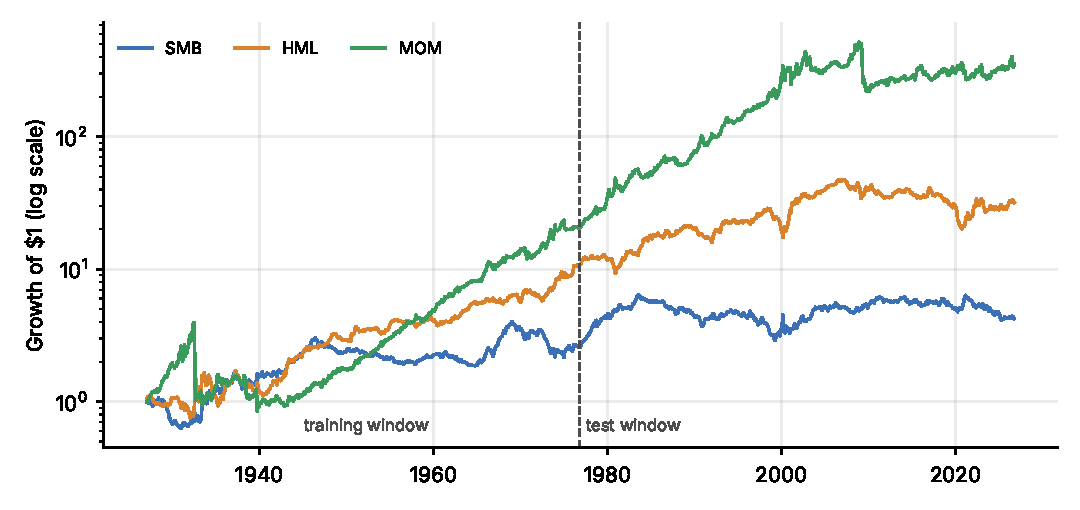
\includegraphics[width=0.92\textwidth]{cumulative_factor_returns_monthly.pdf}
\caption{Growth of \$1 in each monthly factor, January 1927 -- September 2026 (log scale). Final values: \SMB{} \$4.2, \HML{} \$31.9, \MOM{} \$357.6. The dashed line marks the train/test split.}
\end{figure}

\subsection{Monthly}
\begin{center}
\resizebox{\textwidth}{!}{%
\begin{tabular}{llrrrrrrrrrrrr}
\toprule
Window & Factor & Mean & SD & Min & Median & Max & Skew & Ex.\ kurt & AC(1) & \% $>0$ & Ann.\ mean & Ann.\ SD & $t$ \\
\midrule
Full & \SMB & 0.17 & 3.15 & $-17.39$ & 0.07 & 35.96 & 1.78 & 17.8 & 0.05 & 50.8 & 2.02 & 10.92 & 1.85 \\
(1{,}197) & \HML & 0.35 & 3.56 & $-13.83$ & 0.15 & 35.52 & 2.04 & 17.8 & 0.20 & 52.5 & 4.21 & 12.32 & 3.41 \\
 & \MOM & 0.62 & 4.70 & $-52.61$ & 0.80 & 18.05 & $-3.02$ & 27.4 & 0.07 & 62.6 & 7.41 & 16.27 & 4.55 \\
\midrule
Train & \SMB & 0.21 & 3.35 & $-9.75$ & $-0.06$ & 35.96 & 2.71 & 24.1 & 0.10 & 49.2 & 2.53 & 11.60 & 1.54 \\
(598) & \HML & 0.47 & 3.99 & $-13.19$ & 0.19 & 35.52 & 2.81 & 21.4 & 0.22 & 53.8 & 5.67 & 13.81 & 2.90 \\
 & \MOM & 0.66 & 5.00 & $-52.61$ & 0.90 & 15.78 & $-4.13$ & 37.2 & 0.09 & 63.7 & 7.88 & 17.32 & 3.21 \\
\midrule
Test & \SMB & 0.13 & 2.95 & $-17.39$ & 0.13 & 21.34 & 0.39 & 6.5 & $-0.02$ & 52.4 & 1.52 & 10.20 & 1.05 \\
(599) & \HML & 0.23 & 3.07 & $-13.83$ & 0.07 & 12.86 & 0.14 & 2.1 & 0.16 & 51.3 & 2.74 & 10.62 & 1.82 \\
 & \MOM & 0.58 & 4.38 & $-34.36$ & 0.76 & 18.05 & $-1.34$ & 9.9 & 0.05 & 61.4 & 6.95 & 15.16 & 3.24 \\
\bottomrule
\end{tabular}}
\end{center}

\subsection{Weekly}
\begin{center}
\resizebox{\textwidth}{!}{%
\begin{tabular}{llrrrrrrrrrrrr}
\toprule
Window & Factor & Mean & SD & Min & Median & Max & Skew & Ex.\ kurt & AC(1) & \% $>0$ & Ann.\ mean & Ann.\ SD & $t$ \\
\midrule
Full & \SMB & 0.03 & 1.28 & $-9.70$ & 0.01 & 10.17 & 0.08 & 6.8 & 0.06 & 50.3 & 1.43 & 9.20 & 1.56 \\
(5{,}212) & \HML & 0.08 & 1.51 & $-12.45$ & 0.03 & 15.47 & 0.83 & 11.3 & 0.05 & 51.2 & 4.02 & 10.92 & 3.69 \\
 & \MOM & 0.13 & 1.98 & $-19.71$ & 0.23 & 12.65 & $-1.39$ & 11.3 & 0.07 & 58.0 & 6.83 & 14.27 & 4.79 \\
\midrule
Train & \SMB & 0.03 & 1.26 & $-9.06$ & $-0.02$ & 10.17 & 0.41 & 10.1 & 0.11 & 48.9 & 1.70 & 9.11 & 1.32 \\
(2{,}606) & \HML & 0.10 & 1.55 & $-12.45$ & 0.03 & 15.47 & 1.22 & 14.9 & 0.07 & 51.2 & 5.11 & 11.17 & 3.24 \\
 & \MOM & 0.13 & 1.91 & $-19.71$ & 0.22 & 8.16 & $-1.70$ & 13.9 & 0.13 & 58.1 & 6.51 & 13.81 & 3.34 \\
\midrule
Test & \SMB & 0.02 & 1.29 & $-9.70$ & 0.06 & 6.71 & $-0.22$ & 3.9 & 0.01 & 51.6 & 1.17 & 9.29 & 0.89 \\
(2{,}606) & \HML & 0.06 & 1.48 & $-8.79$ & 0.03 & 10.87 & 0.38 & 6.9 & 0.03 & 51.2 & 2.93 & 10.66 & 1.95 \\
 & \MOM & 0.14 & 2.04 & $-15.79$ & 0.24 & 12.65 & $-1.12$ & 9.2 & 0.02 & 58.0 & 7.15 & 14.72 & 3.44 \\
\bottomrule
\end{tabular}}
\end{center}

\subsection{Correlations}
\begin{center}
\begin{tabular}{lccc c ccc}
\toprule
 & \multicolumn{3}{c}{Monthly} && \multicolumn{3}{c}{Weekly} \\
\cmidrule{2-4}\cmidrule{6-8}
Window & \SMB--\HML & \SMB--\MOM & \HML--\MOM && \SMB--\HML & \SMB--\MOM & \HML--\MOM \\
\midrule
Full & 0.13 & $-0.16$ & $-0.41$ && $-0.01$ & $-0.05$ & $-0.25$ \\
Train & 0.33 & $-0.30$ & $-0.54$ && 0.08 & $-0.08$ & $-0.22$ \\
Test & $-0.17$ & 0.01 & $-0.21$ && $-0.10$ & $-0.02$ & $-0.27$ \\
\bottomrule
\end{tabular}
\end{center}

\subsection{What the statistics show}
\begin{itemize}
\item \textbf{Unequal volatility.} \MOM{} is the most volatile factor (monthly SD 4.70\% vs 3.15\% for \SMB), which by itself makes it top more often under the raw argmax. This is the motivation for the optional volatility scaling.
\item \textbf{Fat tails.} All factors have large excess kurtosis, especially in training; \MOM{} has a strong negative skew from crashes (worst month $-52.6\%$, 1932; $-34.4\%$ in 2009).
\item \textbf{The two halves differ.} Premia are smaller in the test window (\HML{} mean 0.23\% vs 0.47\% monthly), tails are thinner, and correlations change sign (\SMB--\HML{} 0.33 in training, $-0.17$ in test). A model estimated on the first half is evaluated on a period with different behaviour.
\item \textbf{Weak serial dependence.} First-order autocorrelations are small (mostly 0.0--0.2), so period-to-period predictability in returns themselves is limited.
\end{itemize}

%==========================================================================
\section{The encoded observation sequence}\label{sec:encoding}

\subsection{Top-factor counts and shares}
\begin{center}
\begin{tabular}{ll rrr c rrr}
\toprule
 & & \multicolumn{3}{c}{Count} && \multicolumn{3}{c}{Share} \\
\cmidrule{3-5}\cmidrule{7-9}
Dataset & Window & \SMB & \HML & \MOM && \SMB & \HML & \MOM \\
\midrule
Monthly & Full & 314 & 354 & 529 && 0.262 & 0.296 & 0.442 \\
 & Train & 146 & 174 & 278 && 0.244 & 0.291 & 0.465 \\
 & Test & 168 & 180 & 251 && 0.280 & 0.301 & 0.419 \\
\midrule
Weekly & Full & 1{,}461 & 1{,}585 & 2{,}166 && 0.280 & 0.304 & 0.416 \\
 & Train & 690 & 796 & 1{,}120 && 0.265 & 0.305 & 0.430 \\
 & Test & 771 & 789 & 1{,}046 && 0.296 & 0.303 & 0.401 \\
\bottomrule
\end{tabular}
\end{center}
The training shares are the frequencies $\hat p_k$ used to build the starting emission matrix and the lift check.

\subsection{Persistence of the raw top factor}
\begin{center}
\begin{tabular}{l ccc c c}
\toprule
 & \multicolumn{3}{c}{Average run length (periods)} && Share of periods \\
\cmidrule{2-4}
Dataset, window & \SMB & \HML & \MOM && top factor changes \\
\midrule
Monthly, train & 1.40 & 1.58 & 1.93 && 0.598 \\
Monthly, test & 1.47 & 1.58 & 1.77 && 0.617 \\
Weekly, train & 1.58 & 1.54 & 2.03 && 0.578 \\
Weekly, test & 1.49 & 1.54 & 1.76 && 0.624 \\
\bottomrule
\end{tabular}
\end{center}
With three roughly equally likely outcomes and no memory, the top factor would change about two-thirds of the time; the observed 58--62\% indicates at most mild persistence in the raw sequence.

\subsection{Transition counts (full sample)}
Rows: top factor this period; columns: top factor next period.
\[
N_{\text{monthly}}=
\begin{pmatrix}
96 & 78 & 140\\
78 & 130 & 146\\
140 & 145 & 243
\end{pmatrix},
\qquad
N_{\text{weekly}}=
\begin{pmatrix}
506 & 428 & 527\\
408 & 556 & 621\\
547 & 601 & 1{,}017
\end{pmatrix}.
\]
Training-window counts are given in the build log (Section 4.4).

\subsection{Ties and margins}
\begin{center}
\begin{tabular}{lccc}
\toprule
 & Exact ties for top & Median margin, top vs second (pp) & Margin $<0.1$ pp \\
\midrule
Monthly & 4 of 1{,}197 & 1.82 & 3.8\% of months \\
Weekly & 1 of 5{,}212 & 0.77 & 8.1\% of weeks \\
\bottomrule
\end{tabular}
\end{center}
Ties are too rare to matter. Near-ties are more common weekly: about one week in twelve is decided by less than 0.1 percentage point, one reason the weekly top factor is noisier.

\subsection{Top-factor shares by decade (monthly)}
\begin{center}
\begin{tabular}{lrrrr}
\toprule
Decade & \SMB & \HML & \MOM & Months \\
\midrule
1920s (from 1927) & 0.14 & 0.25 & 0.61 & 36 \\
1930s & 0.25 & 0.27 & 0.48 & 120 \\
1940s & 0.32 & 0.33 & 0.35 & 120 \\
1950s & 0.23 & 0.27 & 0.50 & 120 \\
1960s & 0.22 & 0.33 & 0.45 & 120 \\
1970s & 0.28 & 0.25 & 0.47 & 120 \\
1980s & 0.21 & 0.37 & 0.42 & 120 \\
1990s & 0.27 & 0.30 & 0.43 & 120 \\
2000s & 0.32 & 0.28 & 0.40 & 120 \\
2010s & 0.30 & 0.28 & 0.42 & 120 \\
2020s (to Sep 2026) & 0.26 & 0.30 & 0.44 & 81 \\
\bottomrule
\end{tabular}
\end{center}
\MOM{} tops most often in every decade except the 1940s, where the three factors are nearly level.

%==========================================================================
\section{Consistency checks}\label{sec:checks}
\sloppy

\begin{itemize}
\item \textbf{Momentum construction.} Compounding the daily momentum file into calendar months and comparing with the monthly momentum file over 1{,}197 months gives a correlation of 0.928 and a mean absolute difference of 0.93 pp per month. The series agree in direction and size but are not identical, as expected from their different sort frequencies and look-back windows. Weekly results therefore use daily-constructed momentum and monthly results use monthly-constructed momentum.
\item \textbf{Week alignment.} Momentum days are assigned to French's weekly periods rather than to calendar weeks, so weekly \SMB, \HML{} and \MOM{} cover the same trading days. The first kept week (ending 6 November 1926) has four momentum days (from 3 November); the 3-factor week may include one earlier trading day, a negligible mismatch in one of 5{,}212 weeks.
\item \textbf{No look-ahead in cleaning.} All cleaning steps are row-wise or use only past data (the volatility-scaling window is lagged), so the test window is untouched by training-period choices other than the split date.
\end{itemize}

%==========================================================================
\section{Pilot data (not used in final results)}
S\&P Dow Jones Indices ``Performance Graph'' exports of daily index levels: S\&P 500 Value, S\&P 500/S\&P SmallCap 600 130/30 and S\&P 500 Momentum (one-year and ten-year versions).
\begin{itemize}
\item One-year momentum export: 252 days (Oct 2025 -- Oct 2026); overlap with the other two gave 53 weeks, too few to fit.
\item Ten-year exports: 2{,}534--2{,}535 days each (30 Sep 2016 -- 29 Oct 2026); converted to daily returns, compounded into weeks ending Friday, giving 526 weeks (263 train / 263 test).
\item Abandoned because the indices are long-only and highly correlated (weekly $\rho=0.75$--$0.89$), so the top index mostly reflected market direction, and the 130/30 index is not a size factor (build log, Section~7).
\end{itemize}

%==========================================================================
\appendix
\section{Reproduction}
\sloppy
The cleaned datasets are \texttt{data/clean/sta348\_factor\_data\_monthly.csv} and \texttt{\_weekly.csv} (columns: date, \SMB, \HML, \MOM{} in decimals, \texttt{top\_factor}, \texttt{top\_code}, \texttt{window}). The statistics in this document are produced by
\begin{verbatim}
python code/analysis/datadiag.py code \
    data/raw_ken_french/F-F_Research_Data_Factors_CSV.zip \
    data/raw_ken_french/F-F_Momentum_Factor_CSV.zip \
    data/raw_ken_french/F-F_Research_Data_Factors_weekly.csv \
    data/raw_ken_french/F-F_Momentum_Factor_daily.csv
\end{verbatim}
which uses the same loading functions as the model (\texttt{read\_french\_daily}, \texttt{load\_french}, \texttt{make\_observations} in \texttt{sta348\_hmm\_v1.py}).

\end{document}
